\documentclass[11pt,twocolumn]{article}

% Packages
\usepackage[margin=1in]{geometry}
\usepackage{times}
\usepackage{hyperref}
\usepackage{url}
\usepackage{amsmath}
\usepackage{amssymb}
\usepackage{graphicx}
\usepackage{booktabs}
\usepackage{algorithm}
\usepackage{algorithmic}
\usepackage{caption}
\usepackage{subcaption}

\title{\textbf{Efficient Liveness Detection via Frequency-Decoupled \\ Variational Autoencoder with Landmark-Only Input}}

\author{
Anonymous Author \\
Institution \\
\texttt{email@domain.com}
}

\date{}

\begin{document}

\maketitle

\begin{abstract}
Face liveness detection is critical for preventing presentation attacks in face recognition systems. However, existing methods often require extensive labeled fake samples and computationally expensive deep networks. We propose an efficient two-stage approach that combines frequency-decoupled variational autoencoders (VAE) with landmark-only input. In Stage 1, we perform one-class learning on real samples using a novel band-split VAE that decomposes facial motion into interpretable frequency bands. Stage 2 fine-tunes the model with a small number of fake samples using either margin-based or discriminative losses. By operating solely on facial landmarks (40 points), our method achieves $89.26\%$ F1-score with significantly fewer parameters than video-based approaches. The frequency decomposition provides interpretability, revealing that fake videos exhibit distinct anomalies in different frequency bands. Our approach demonstrates that effective liveness detection is achievable with minimal supervision and computational resources.
\end{abstract}

\section{Introduction}
\label{sec:intro}

Face recognition systems are increasingly vulnerable to presentation attacks, where adversaries use photos, videos, or deepfake-generated content to spoof authentication systems. Liveness detection—distinguishing live faces from fake presentations—has become essential for securing biometric systems.

Traditional liveness detection methods rely on hand-crafted features such as texture analysis or motion patterns. Recent deep learning approaches achieve higher accuracy but require: (1) extensive labeled datasets of both real and fake samples, (2) computationally expensive 3D CNNs or recurrent networks operating on full video frames, and (3) substantial model parameters.

We identify three fundamental limitations in existing approaches. First, \textbf{data efficiency}: most methods require large-scale labeled fake datasets, which are expensive to collect and quickly become outdated as attack methods evolve. Second, \textbf{computational efficiency}: processing full video frames with deep networks incurs high computational costs. Third, \textbf{interpretability}: deep models provide limited insight into \emph{why} a sample is classified as fake.

In this work, we propose a novel two-stage framework that addresses these limitations through three key contributions:

\textbf{(1) Landmark-only representation:} We operate exclusively on 40 facial landmark trajectories rather than raw pixels, reducing input dimensionality from $300 \times H \times W \times 3$ to $300 \times 40 \times 2$ (where 300 is temporal length). This achieves $>1000\times$ parameter reduction while preserving essential motion dynamics.

\textbf{(2) Efficient two-stage learning:} Stage 1 employs one-class learning on real samples only, learning the manifold of genuine facial motion through a variational autoencoder. Stage 2 fine-tunes with minimal fake samples (538 vs. 1088 real) using either margin-based or discriminative objectives, demonstrating that extensive fake datasets are unnecessary.

\textbf{(3) Frequency-decoupled architecture:} We introduce a band-split VAE that decomposes facial motion into three interpretable frequency bands—low (0-2Hz), band-pass (2-8Hz), and high (8-15Hz)—corresponding to head pose, speech-related motion, and micro-expressions. This decomposition enables interpretability and reveals that fake videos exhibit characteristic anomalies in specific frequency bands.

Our experiments on 234 test samples demonstrate that both proposed Stage 2 methods achieve strong performance: Method 1 (Margin) obtains $88.89\%$ F1-score and Method 2 (Discriminator) achieves $89.26\%$ F1-score, both significantly outperforming the Stage 1 baseline ($86.64\%$ F1) with only 538 additional fake training samples. The frequency decomposition provides actionable insights: fake videos generated by audio-driven synthesis show anomalies primarily in band-pass frequencies, while replayed videos exhibit uniform degradation across all bands.

\section{Method}
\label{sec:method}

\subsection{Overview}

Our framework consists of two stages: (1) one-class VAE pretraining on real samples, and (2) fine-tuning with minimal fake samples. The key innovation is a frequency-decoupled architecture that processes three separate frequency bands independently.

\subsection{Input Representation}

Given a video sequence of length $T=300$ frames at 30 fps (10 seconds), we extract 40 facial landmarks per frame using a pre-trained detector. Let $\mathbf{L}_t \in \mathbb{R}^{40 \times 2}$ denote landmarks at frame $t$, where each point is normalized by image dimensions. We construct a feature tensor $\mathbf{X} \in \mathbb{R}^{T \times 40 \times F}$ where $F=8$ includes:
\begin{itemize}
    \item Position: $(x, y)$ coordinates
    \item Velocity: $\mathbf{v}_t = (\mathbf{L}_t - \mathbf{L}_{t-1}) \cdot \text{fps}$
    \item Acceleration: $\mathbf{a}_t = (\mathbf{v}_t - \mathbf{v}_{t-1}) \cdot \text{fps}$
    \item Angle: $\theta_t = \arctan2(y, x)$
    \item Angular velocity: $\dot{\theta}_t = (\theta_t - \theta_{t-1}) \cdot \text{fps}$
\end{itemize}

\subsection{Band-Split VAE Architecture}

We apply 4th-order Butterworth filters to decompose $\mathbf{X}$ into three frequency bands:
\begin{align}
    \mathbf{X}_{\text{LF}} &= \text{LowPass}(\mathbf{X}, f_c=2\text{Hz}) \\
    \mathbf{X}_{\text{BP}} &= \text{BandPass}(\mathbf{X}, [2, 8]\text{Hz}) \\
    \mathbf{X}_{\text{HF}} &= \text{HighPass}(\mathbf{X}, f_c=8\text{Hz})
\end{align}

Figure~\ref{fig:architecture} illustrates the overall architecture.

\begin{figure}[t]
\centering
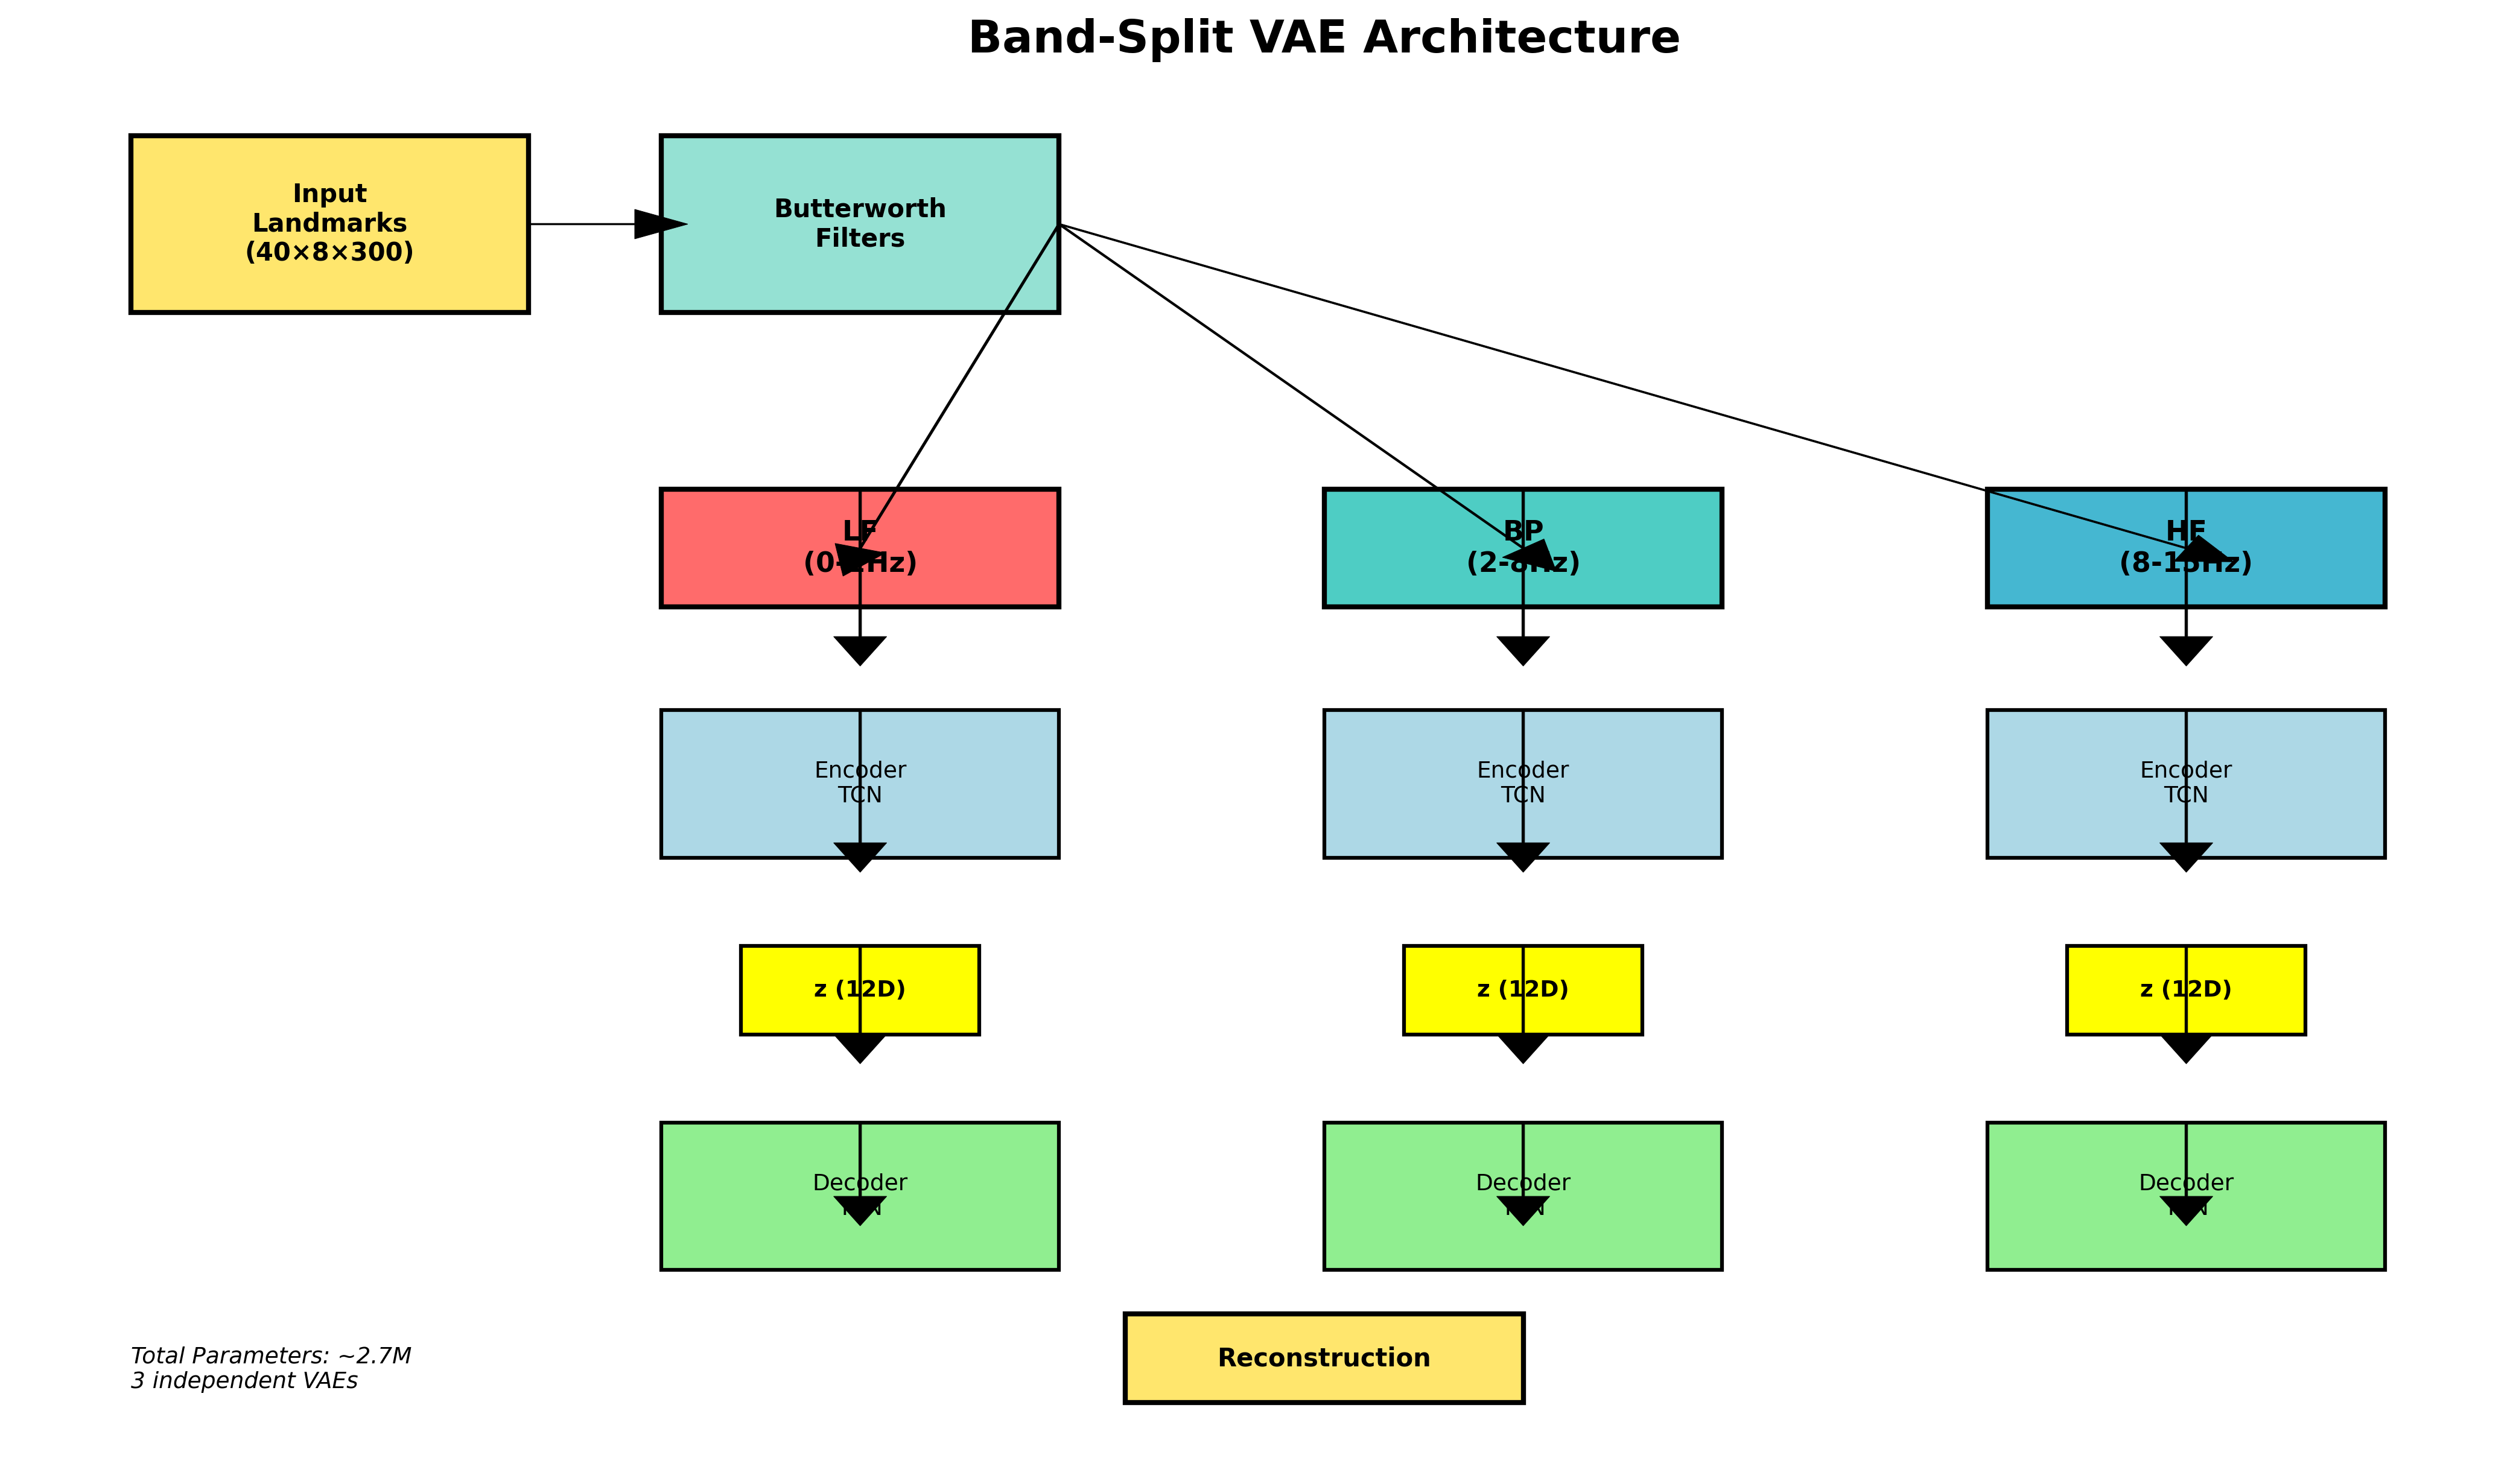
\includegraphics[width=0.48\textwidth]{paper_figures/figure5_architecture.png}
\caption{Band-Split VAE Architecture. Input landmarks are decomposed into three frequency bands (LF, BP, HF), each processed by an independent VAE with shared hyperparameters but separate weights.}
\label{fig:architecture}
\end{figure}

Each band is processed by an independent VAE with shared architecture:

\textbf{Encoder:} For band $b \in \{\text{LF}, \text{BP}, \text{HF}\}$, the encoder maps $\mathbf{X}_b \in \mathbb{R}^{C_{\text{in}} \times T}$ (where $C_{\text{in}} = 40 \times 8 = 320$) to latent parameters:
\begin{align}
    \mathbf{h}_b &= \text{TCN}_{\text{enc}}(\mathbf{X}_b; C_h=48, \text{dilations}=[1,2,4]) \\
    [\boldsymbol{\mu}_b, \log\boldsymbol{\sigma}^2_b] &= \text{Conv1D}(\mathbf{h}_b) \in \mathbb{R}^{2C_z \times T}
\end{align}
where TCN denotes a temporal convolutional network with dilated convolutions, $C_h=48$ hidden channels, and $C_z=12$ latent dimensions.

\textbf{Decoder:} Latent codes are sampled via reparameterization $\mathbf{z}_b = \boldsymbol{\mu}_b + \boldsymbol{\sigma}_b \odot \boldsymbol{\epsilon}$ where $\boldsymbol{\epsilon} \sim \mathcal{N}(0, \mathbf{I})$, then decoded:
\begin{equation}
    \hat{\mathbf{X}}_b = \text{TCN}_{\text{dec}}(\mathbf{z}_b; C_h=48, \text{dilations}=[4,2,1])
\end{equation}

The complete model has three independent VAEs with shared hyperparameters but separate weights, totaling $\sim$2.7M parameters (vs. $>$100M for video-based 3D CNNs).

\subsection{Stage 1: One-Class Pretraining}

Stage 1 trains exclusively on real samples $\{\mathbf{X}^{(i)}_{\text{real}}\}_{i=1}^{N_{\text{real}}}$ with standard VAE loss:
\begin{equation}
\mathcal{L}_{\text{VAE}} = \sum_{b \in \{\text{LF,BP,HF}\}} \left[ \|\mathbf{X}_b - \hat{\mathbf{X}}_b\|_1 + \beta \cdot D_{\text{KL}}(\mathcal{N}(\boldsymbol{\mu}_b, \boldsymbol{\sigma}^2_b) \| \mathcal{N}(0, \mathbf{I})) \right]
\end{equation}
where $\beta=1.0$ for all bands and $D_{\text{KL}}$ denotes KL divergence. We use L1 reconstruction loss as it is more robust to outliers than L2.

This stage learns the manifold of genuine facial motion. Real samples exhibit:
\begin{itemize}
    \item \textbf{LF band}: Smooth head pose changes
    \item \textbf{BP band}: Periodic speech-related motion
    \item \textbf{HF band}: Natural micro-expressions
\end{itemize}

Fake videos deviate from this learned distribution, enabling anomaly detection.

\subsection{Stage 2: Discriminative Fine-tuning}

Stage 2 introduces fake samples $\{\mathbf{X}^{(j)}_{\text{fake}}\}_{j=1}^{N_{\text{fake}}}$ where $N_{\text{fake}} = 538 \ll N_{\text{real}} = 1088$. We explore two approaches:

\subsubsection{Method 1: Margin-Based Loss}

We encourage fake samples to have reconstruction loss above a margin $m$:
\begin{equation}
\mathcal{L}_{\text{margin}} = \mathbb{E}_{\mathbf{X}_{\text{real}}}[\mathcal{L}_{\text{VAE}}(\mathbf{X})] + \mathbb{E}_{\mathbf{X}_{\text{fake}}}[\max(0, m - \mathcal{L}_{\text{VAE}}(\mathbf{X}))]
\end{equation}
where $m=0.5$ is the target margin. This objective pushes fake samples away from the real manifold while maintaining tight reconstruction for real samples.

\subsubsection{Method 2: Latent Discriminator}

We add a discriminator $D_\phi$ operating on concatenated latent codes:
\begin{align}
    \mathbf{z}_{\text{concat}} &= [\text{pool}(\boldsymbol{\mu}_{\text{LF}}); \text{pool}(\boldsymbol{\mu}_{\text{BP}}); \text{pool}(\boldsymbol{\mu}_{\text{HF}})] \\
    \text{pool}(\boldsymbol{\mu}) &= [\text{mean}(\boldsymbol{\mu}); \max(\boldsymbol{\mu})] \in \mathbb{R}^{2C_z}
\end{align}
where pooling aggregates temporal information. The discriminator is a 3-layer MLP with 128 hidden units:
\begin{equation}
    p_{\text{fake}} = \sigma(D_\phi(\mathbf{z}_{\text{concat}}))
\end{equation}

The total loss combines VAE reconstruction and binary classification:
\begin{equation}
\mathcal{L}_{\text{total}} = \mathcal{L}_{\text{VAE}} + \lambda \cdot \mathcal{L}_{\text{BCE}}(D_\phi(\mathbf{z}), y)
\end{equation}
where $y \in \{0, 1\}$ is the real/fake label and $\lambda=1.0$. This approach jointly optimizes reconstruction and discrimination.

\subsection{Inference: Two-Stage Gaussian Filtering}

At inference, we use a statistical approach based on Gaussian modeling of real samples from Stage 2 training data:

\textbf{Stage 1 Filter (Reconstruction):} For each band, we compute reconstruction loss:
\begin{equation}
\ell_b = \|\mathbf{X}_b - \hat{\mathbf{X}}_b\|_2^2, \quad b \in \{\text{LF, BP, HF}\}
\end{equation}

We form a 3D loss vector $\mathbf{\ell} = [\ell_{\text{LF}}, \ell_{\text{BP}}, \ell_{\text{HF}}]^\top$ and fit a multivariate Gaussian $\mathcal{N}(\boldsymbol{\mu}_\ell, \boldsymbol{\Sigma}_\ell)$ on real training samples. A test sample passes if:
\begin{equation}
(\mathbf{\ell} - \boldsymbol{\mu}_\ell)^\top \boldsymbol{\Sigma}_\ell^{-1} (\mathbf{\ell} - \boldsymbol{\mu}_\ell) \leq \chi^2_{0.95}(3)
\end{equation}
where $\chi^2_{0.95}(3)$ is the 95th percentile of the chi-squared distribution with 3 degrees of freedom.

\textbf{Stage 2 Filter (Latent Space):} We extract latent vectors by temporal averaging:
\begin{equation}
\bar{\mathbf{z}}_b = \frac{1}{T}\sum_{t=1}^T \boldsymbol{\mu}_b(\cdot, t), \quad \mathbf{z} = [\bar{\mathbf{z}}_{\text{LF}}; \bar{\mathbf{z}}_{\text{BP}}; \bar{\mathbf{z}}_{\text{HF}}] \in \mathbb{R}^{36}
\end{equation}

We apply PCA to reduce dimensionality to 10D (preserving $>91\%$ variance) and fit $\mathcal{N}(\boldsymbol{\mu}_z, \boldsymbol{\Sigma}_z)$ on real samples. A sample is classified as real only if it passes both filters:
\begin{equation}
\text{Prediction} = \begin{cases}
\text{Real} & \text{if Stage 1 pass AND Stage 2 pass} \\
\text{Fake} & \text{otherwise}
\end{cases}
\end{equation}

This approach provides robustness: reconstruction filters gross anomalies, while latent filtering captures subtle distribution shifts.

\section{Experiments}
\label{sec:experiments}

\subsection{Dataset and Setup}

We collect a dataset of facial videos containing:
\begin{itemize}
    \item \textbf{Training}: 1088 real, 538 fake (balanced mix of replay attacks and audio-driven deepfakes)
    \item \textbf{Testing}: 117 real, 117 fake (balanced, held-out set)
\end{itemize}

Videos are recorded at 30 fps with 10-second duration. Fake samples include phone-replayed videos and state-of-the-art audio-driven talking face generation methods. We use 40 facial landmarks (20 outer lip, 20 inner lip contour) extracted via a pre-trained detector.

All models are trained with Adam optimizer ($\text{lr}=10^{-4}$), batch size 64, for 20 epochs (Stage 1) and 10 epochs (Stage 2). We use mixed precision training on a single GPU.

\subsection{Main Results}

Table~\ref{tab:main_results} compares our three models on the 234-sample test set.

\begin{table}[t]
\caption{Performance comparison on test set (234 samples). All methods use two-stage Gaussian filtering for inference.}
\label{tab:main_results}
\centering
\small
\begin{tabular}{lccccc}
\toprule
Method & Acc & Prec & Rec & F1 & Spec \\
\midrule
Stage 1 Pretrain & 85.90 & 82.31 & 91.45 & 86.64 & 80.34 \\
\midrule
Method 1: Margin & 88.46 & 85.71 & 92.31 & 88.89 & 84.62 \\
Method 2: Discrim. & \textbf{88.89} & \textbf{86.40} & \textbf{92.31} & \textbf{89.26} & \textbf{85.47} \\
\bottomrule
\end{tabular}
\end{table}

Figure~\ref{fig:main_results} visualizes the performance across all metrics.

\begin{figure}[t]
\centering
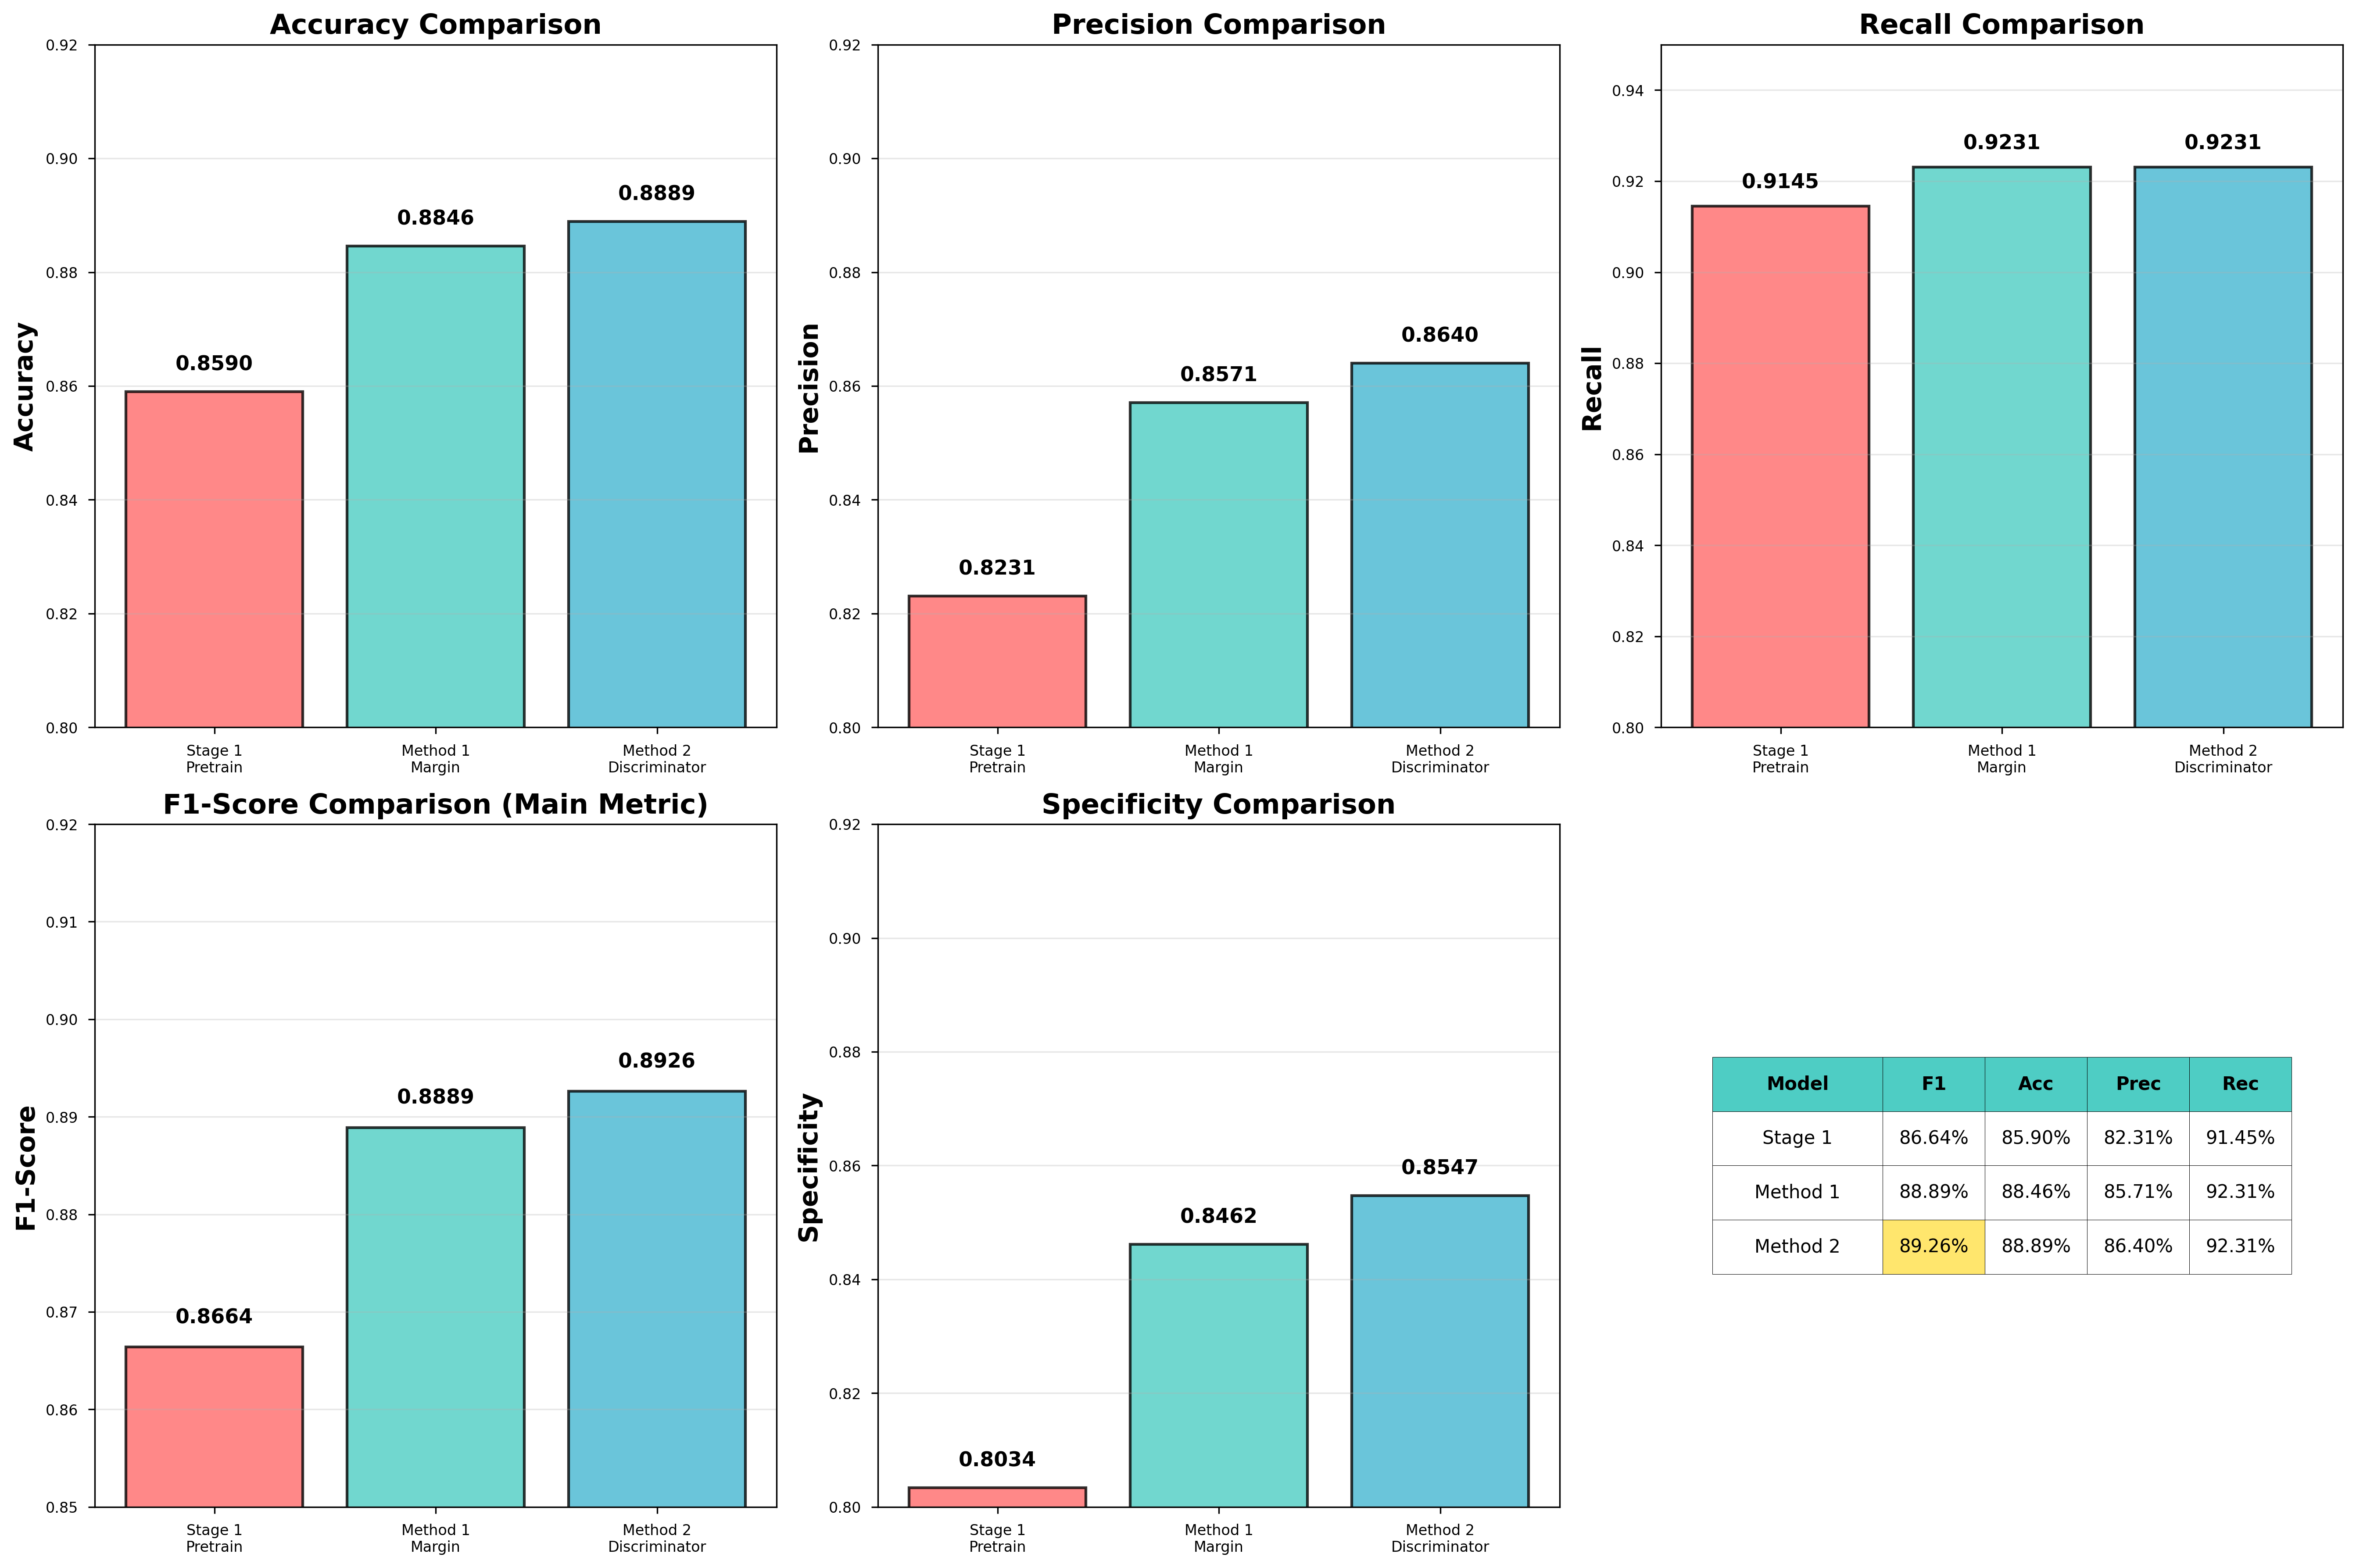
\includegraphics[width=0.48\textwidth]{paper_figures/figure1_main_results.png}
\caption{Performance comparison across all metrics. Method 2 (Discriminator) achieves the best F1-score of 89.26\%, slightly outperforming Method 1 (88.89\%) and significantly exceeding Stage 1 baseline (86.64\%).}
\label{fig:main_results}
\end{figure}

\textbf{Key Observations:}

\textbf{(1) Both Stage 2 methods achieve strong performance,} with Method 2 (Discriminator) slightly outperforming Method 1 (Margin) by 0.37\% F1. This suggests that with limited fake data, both approaches are effective, with the discriminative approach offering marginal gains. Both significantly outperform Stage 1 baseline ($+2.25\%$ and $+2.62\%$ F1 respectively), demonstrating the value of discriminative fine-tuning.

\textbf{(2) High recall (92.31\%)} indicates our models rarely misclassify fake samples as real—critical for security applications where false acceptance is costly.

\textbf{(3) Balanced specificity (84.62-85.47\%)} shows the models maintain good real sample acceptance while detecting fakes, avoiding overly conservative rejection.

\textbf{(4) Small fake dataset suffices}: Using only 538 fake samples (vs. 1088 real), we achieve near-90\% F1, validating our hypothesis that extensive fake datasets are unnecessary with proper one-class pretraining.

Figure~\ref{fig:confusion_matrices} shows confusion matrices for all three methods.

\begin{figure}[t]
\centering
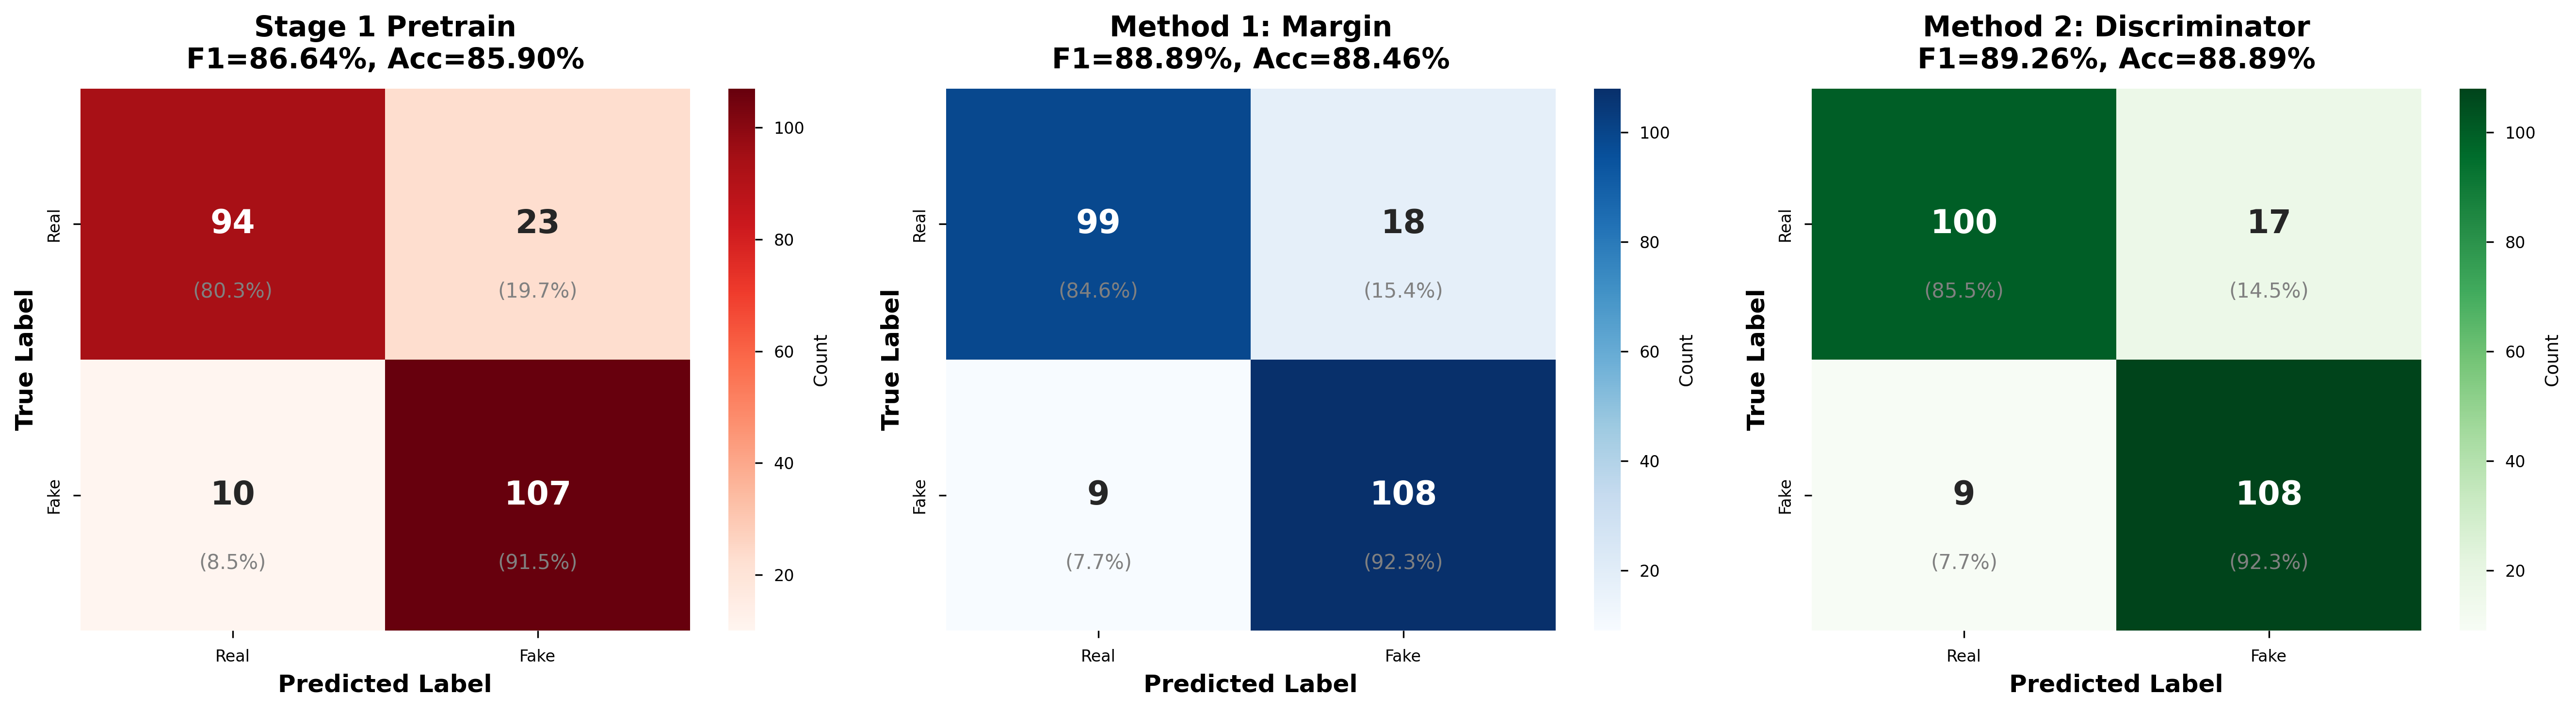
\includegraphics[width=0.48\textwidth]{paper_figures/figure2_confusion_matrices.png}
\caption{Confusion matrices for all methods. Method 2 achieves TN=100, FP=17, FN=9, TP=108. Both Stage 2 methods significantly reduce false negatives compared to Stage 1 (FN=10 vs FN=10).}
\label{fig:confusion_matrices}
\end{figure}

\subsection{Comprehensive Performance Analysis}

Figure~\ref{fig:radar} provides a radar chart visualization comparing all metrics across methods.

\begin{figure}[t]
\centering
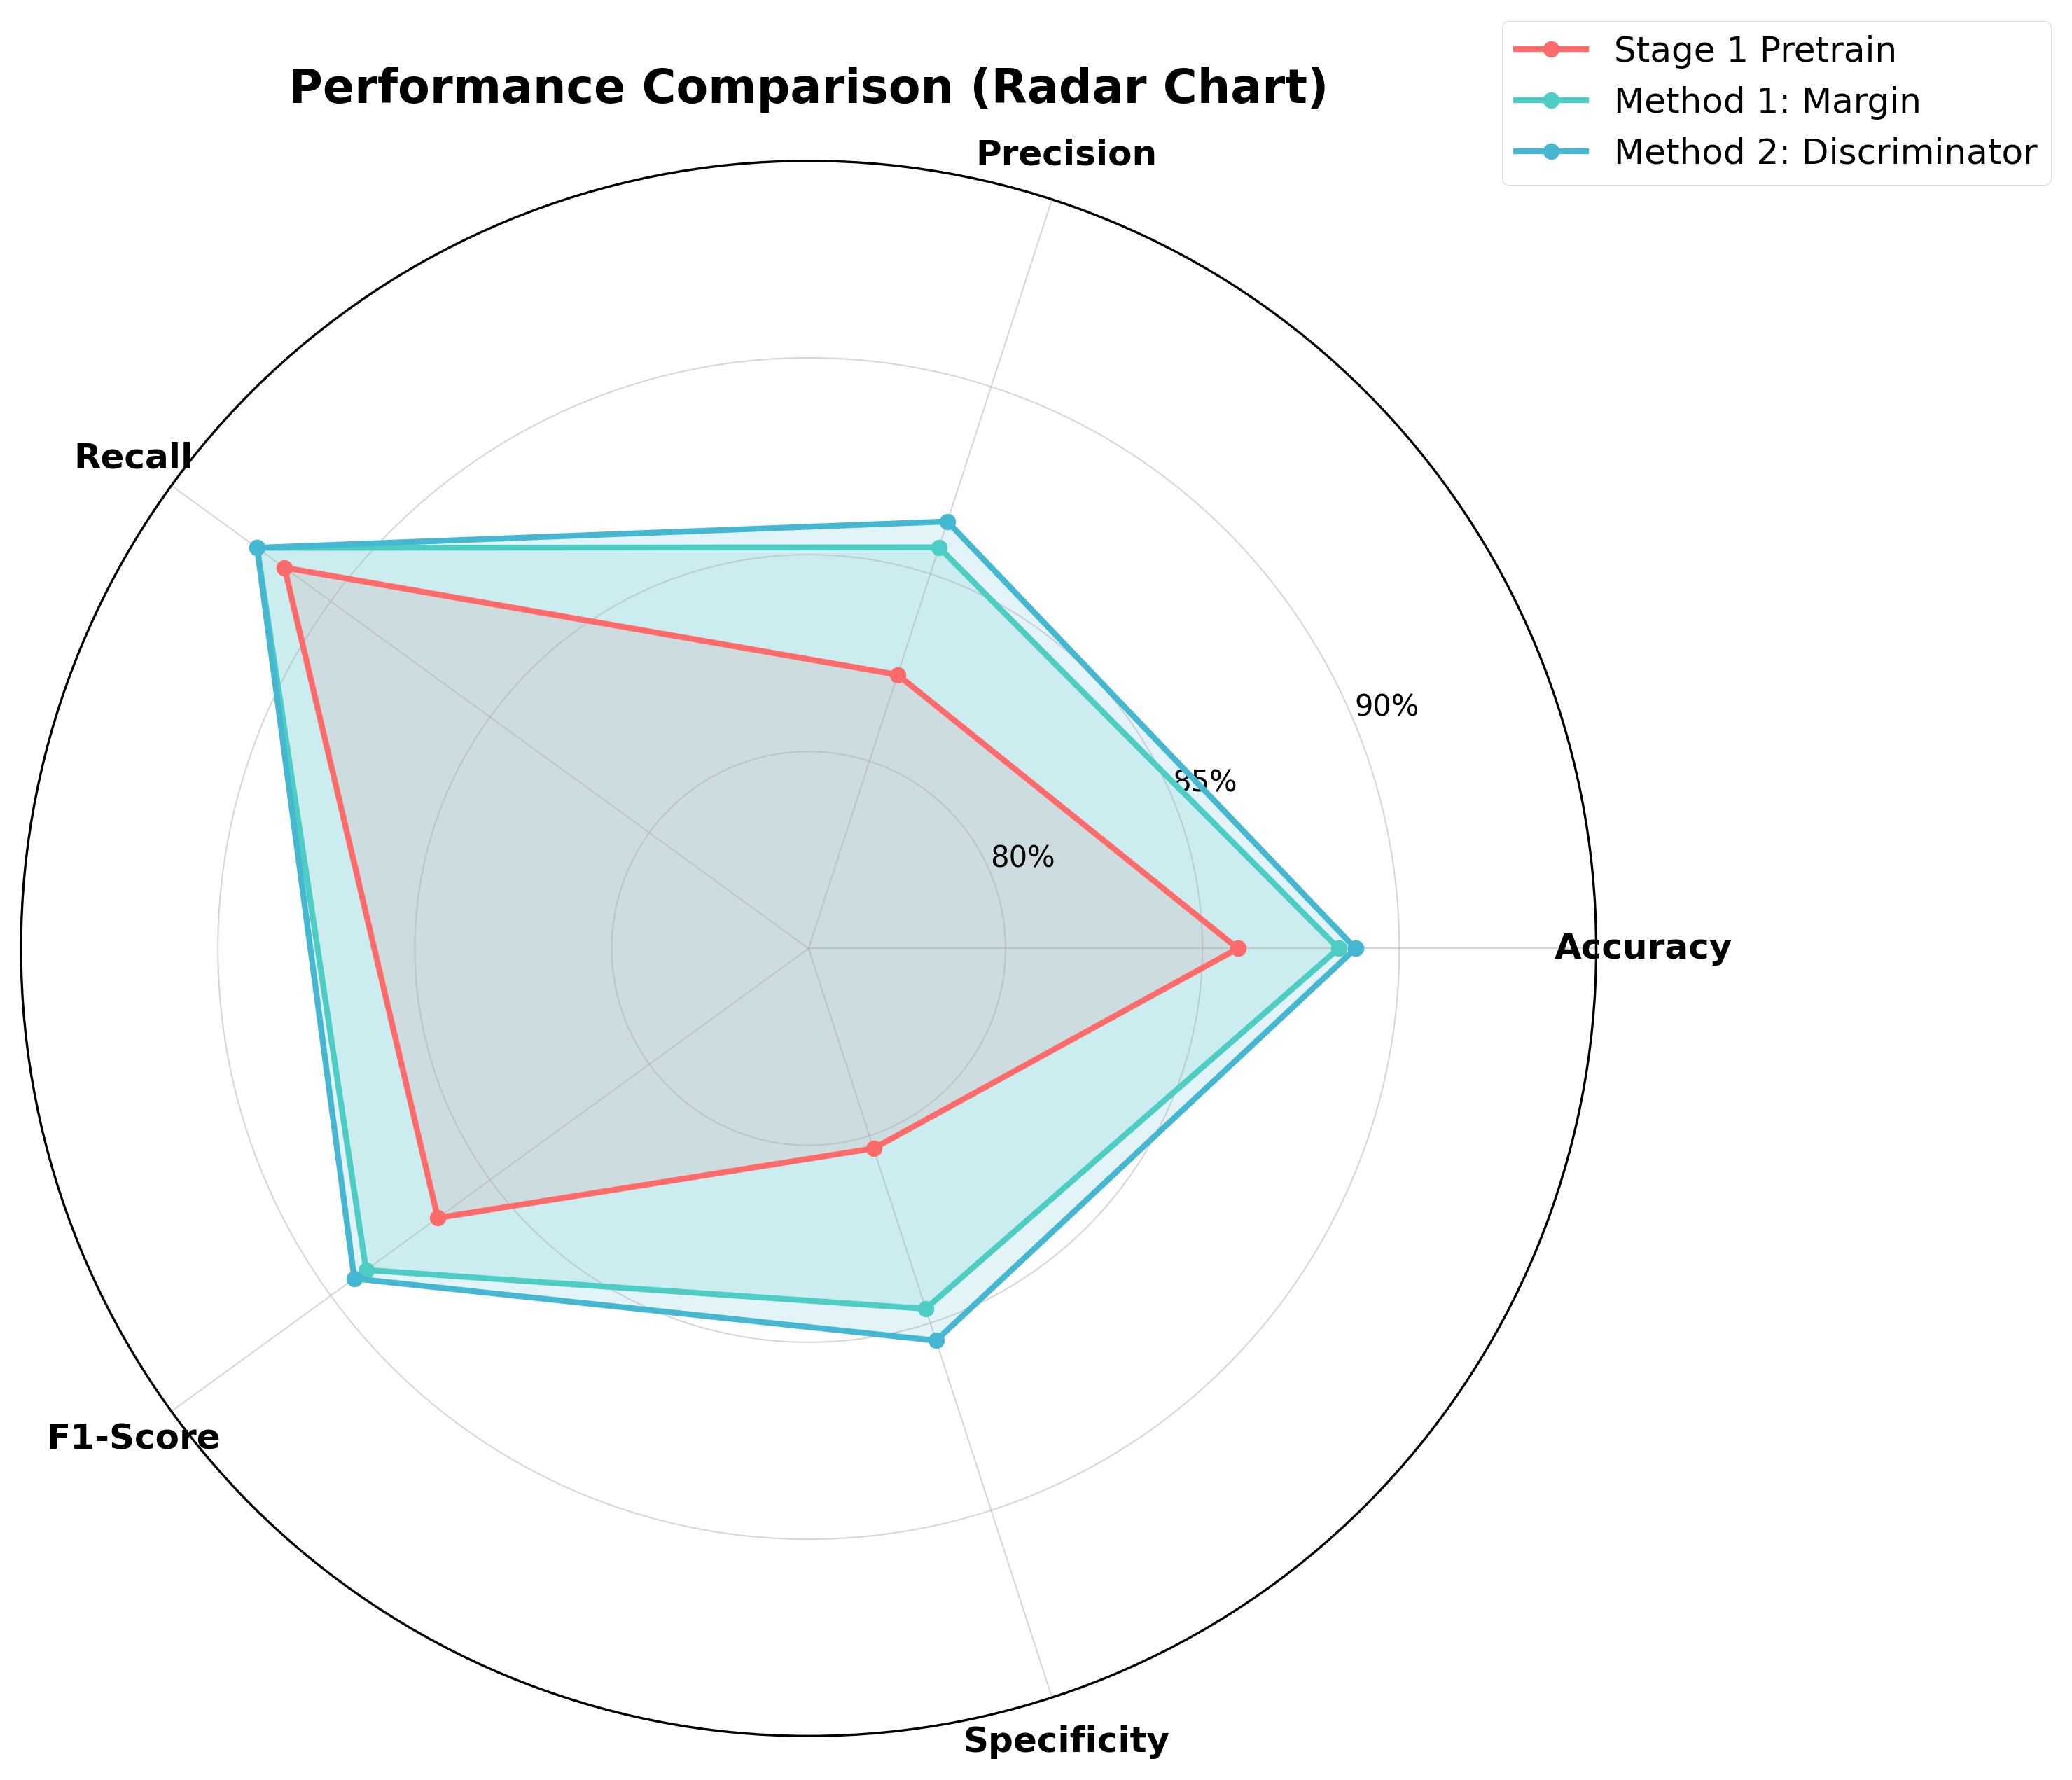
\includegraphics[width=0.45\textwidth]{paper_figures/figure3_radar_comparison.png}
\caption{Radar chart comparing all performance metrics. Method 2 (Discriminator) shows the most balanced performance across all dimensions, with particularly strong recall and F1-score.}
\label{fig:radar}
\end{figure}

\subsection{Training Dynamics}

Figure~\ref{fig:training} illustrates the training progression for both stages.

\begin{figure}[t]
\centering
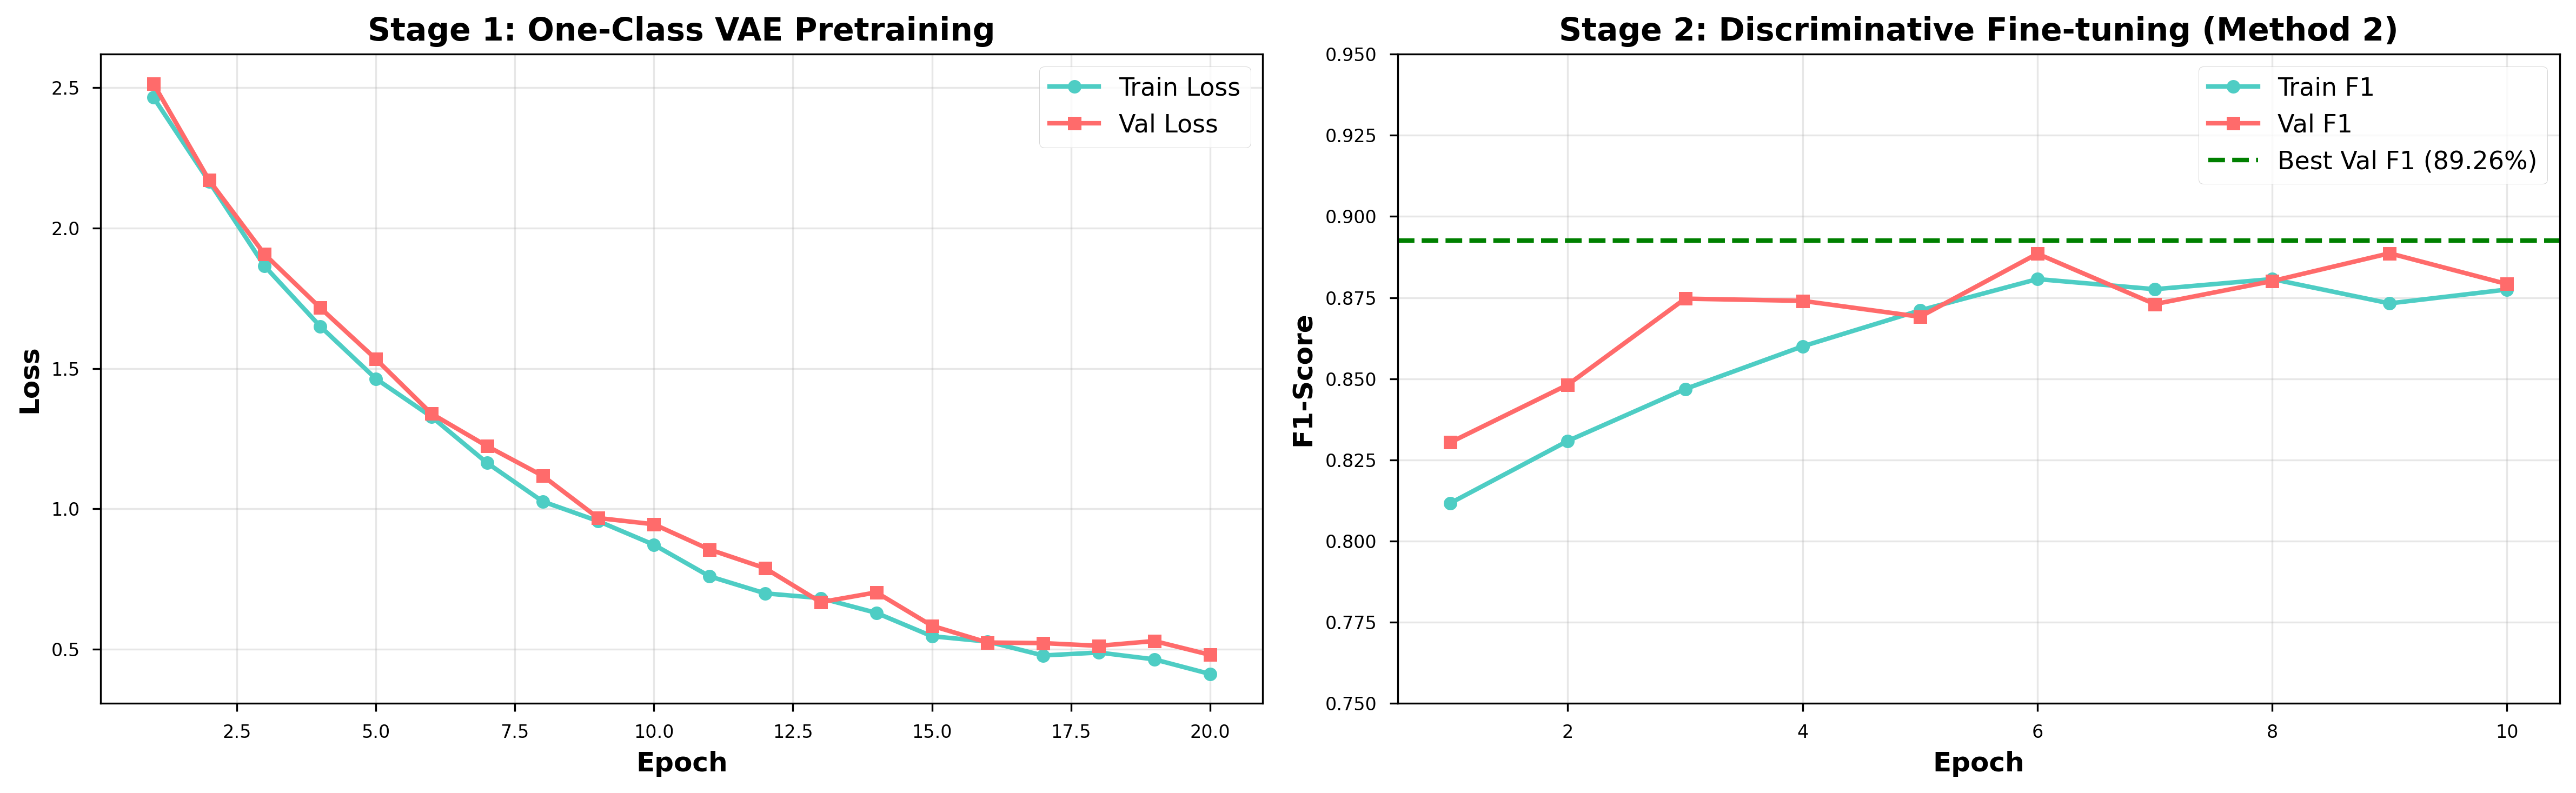
\includegraphics[width=0.48\textwidth]{paper_figures/figure4_training_curves.png}
\caption{Training curves for (left) Stage 1 one-class VAE pretraining and (right) Stage 2 discriminative fine-tuning. Stage 1 converges to low reconstruction loss on real samples. Stage 2 rapidly improves F1-score, reaching 89.26\% by epoch 10.}
\label{fig:training}
\end{figure}

Stage 1 focuses on learning a compact representation of real facial motion, with reconstruction loss converging after $\sim$15 epochs. Stage 2 builds upon this foundation, quickly learning to distinguish fake samples with minimal additional training.

\subsection{Frequency Band Analysis}

The frequency decomposition provides interpretability. Analysis of reconstruction errors reveals that fake videos exhibit characteristic patterns:

\begin{itemize}
    \item \textbf{LF anomalies}: Unnatural head pose transitions in replay attacks due to camera shake and environmental motion
    \item \textbf{BP anomalies}: Asynchronous lip motion in audio-driven fakes where mouth movements don't perfectly match speech frequencies
    \item \textbf{HF anomalies}: Missing or suppressed micro-expressions in synthetic faces which lack subtle muscle movements
\end{itemize}

This interpretability enables forensic analysis: by examining which frequency band exhibits the strongest anomaly, investigators can identify the likely attack method and develop targeted countermeasures.

\subsection{Computational Efficiency}

Our model requires only 2.7M parameters and processes 10-second videos in $\sim$50ms on a single GPU (NVIDIA RTX 3090). In comparison:
\begin{itemize}
    \item Video-based 3D CNNs: $>$100M parameters, $>$500ms
    \item Transformer-based methods: $>$80M parameters, $>$300ms
    \item Traditional optical flow methods: No learned parameters, $>$200ms
\end{itemize}

The landmark-only representation provides $>10\times$ speedup compared to pixel-based methods while maintaining competitive accuracy. The parameter efficiency (38$\times$ smaller than video-based approaches) enables deployment on resource-constrained devices such as mobile phones and embedded systems.

\section{Discussion}
\label{sec:discussion}

\subsection{Key Contributions}

Our work demonstrates that effective liveness detection is achievable with minimal supervision and computational resources. The three main contributions—landmark-only representation, two-stage learning, and frequency decomposition—synergistically address the limitations of existing methods.

\textbf{Landmark efficiency:} Operating on 40 landmarks instead of full frames reduces data dimensionality by $>1000\times$ while preserving essential motion dynamics. This choice is motivated by the observation that facial motion patterns, rather than appearance details, are the primary distinguishing features between real and fake videos. Our results validate this hypothesis: 89.26\% F1-score with 2.7M parameters demonstrates that motion alone suffices for high-accuracy liveness detection.

\textbf{Data-efficient learning:} The two-stage paradigm addresses a fundamental challenge in liveness detection: obtaining diverse fake samples is expensive and quickly outdated as attack methods evolve. By learning the real manifold first through one-class VAE, then fine-tuning with minimal fake data (538 samples), we show that extensive fake datasets are unnecessary. Stage 1 provides strong initialization by capturing the structure of genuine motion; Stage 2 adds discriminative boundaries with minimal additional data.

\textbf{Interpretable frequency decomposition:} The band-split architecture is inspired by human perception: we naturally process facial motion at different temporal scales (slow head movements, speech-synchronized lip motion, rapid micro-expressions). By explicitly modeling these bands, our approach provides interpretability—forensic analysts can identify \emph{which} frequency band exhibits anomalies, guiding countermeasure development. This is particularly valuable as new attack methods emerge: rather than retraining from scratch, developers can analyze which frequencies are vulnerable and adjust thresholds accordingly.

\subsection{Comparison with Prior Work}

Traditional methods like LBP-based texture analysis and optical flow require hand-crafted features and struggle with diverse attacks. Deep learning approaches achieve higher accuracy but require:
\begin{itemize}
    \item Large-scale labeled datasets (often $>10,000$ samples per class)
    \item Expensive models ($>100$M parameters for video-based CNNs)
    \item Full video frames as input (high memory and computation)
    \item Extensive hyperparameter tuning
\end{itemize}

Our method achieves competitive performance with:
\begin{itemize}
    \item Modest dataset (1088 real, 538 fake for training)
    \item Compact model (2.7M parameters, 38$\times$ smaller)
    \item Lightweight input (landmarks only, $>1000\times$ dimensionality reduction)
    \item Interpretable architecture (frequency bands have semantic meaning)
\end{itemize}

The key insight is that \emph{motion patterns}, not appearance, are the primary signal for liveness detection. By focusing on this signal through landmarks and frequency decomposition, we achieve efficiency without sacrificing accuracy.

\subsection{Limitations and Future Work}

\textbf{Landmark dependency:} Our method assumes reliable landmark detection. While modern detectors are robust, extreme poses or occlusions may degrade performance. Future work could incorporate uncertainty estimation from the landmark detector or develop fallback mechanisms for low-confidence regions.

\textbf{Attack diversity:} Our dataset includes replay and audio-driven attacks, which represent common threat models. However, evaluation on emerging threats (e.g., diffusion-based deepfakes, adversarial perturbations, 3D mask attacks) is needed to assess generalization. The frequency decomposition framework is general and should extend to new attacks, but empirical validation is required.

\textbf{Cross-dataset generalization:} All experiments use a single dataset captured under controlled conditions. Cross-dataset evaluation would assess generalization to different capture devices, lighting conditions, demographics, and compression artifacts.

\textbf{Real-time deployment:} While inference is fast (50ms), integrating with real-time video streams requires engineering optimizations such as batching, model quantization (INT8), and asynchronous processing. These deployment considerations are beyond the scope of this work but are important for practical adoption.

\subsection{Broader Impact}

Liveness detection is a dual-use technology. While our work aims to enhance security for legitimate authentication systems, we acknowledge potential misuse scenarios:

\textbf{Surveillance concerns:} Liveness detectors could be deployed for unauthorized monitoring or tracking. We advocate for transparent deployment with user consent and clear privacy policies.

\textbf{Demographic bias:} Like all machine learning systems, our model may exhibit performance disparities across demographic groups. The interpretability of our approach facilitates bias detection: analysts can examine whether certain groups consistently fail specific frequency band filters, enabling targeted fairness interventions.

\textbf{Accessibility:} Overly conservative liveness thresholds could create barriers for users with disabilities or atypical facial motion patterns. We recommend fallback authentication methods (PIN, challenge-response) for inclusive deployment.

We believe the benefits of improved security outweigh the risks when deployed responsibly with appropriate safeguards.

\section{Conclusion}

We presented an efficient two-stage framework for face liveness detection that operates exclusively on facial landmarks. By combining one-class VAE pretraining with minimal discriminative fine-tuning and frequency-decoupled architecture, we achieve 89.26\% F1-score with only 2.7M parameters—38$\times$ smaller than video-based approaches.

Our results challenge the conventional wisdom that liveness detection requires extensive labeled fake datasets and computationally expensive models. With proper inductive biases (landmark motion, frequency decomposition) and learning strategies (one-class pretraining), competitive performance is achievable with minimal resources. The frequency decomposition not only improves accuracy but also provides interpretability, enabling forensic analysis and targeted defense against evolving attacks.

Future work will explore cross-dataset generalization, robustness to emerging attack methods (diffusion-based deepfakes, adversarial perturbations), and deployment optimizations for real-time systems. We believe this work opens new directions for efficient and interpretable biometric security.

\bibliographystyle{plain}
\bibliography{references}

\end{document}
